\chapter{Implementation Acceleration}

\section{Comparison Acceleration with Heap}

\subsection{Heap}

Heap is a widely used data structure in computer science. It is a tree-based data structure, whose node contains a key value for comparing and sorting. For min-heap, the key value of each node is greater than or equal to that of its parent if exists and less than or equal to that of its children also if exists. For max-heap, the situation is just opposite. This is called heap property.

Here we borrowed an example of max-heap from \url{http://en.wikipedia.org/wiki/Heap_(data_structure)}. It can be seen easily that the number in each parent node is greater than or equal to its child nodes if exists.

\begin{figure}[ht]
\centering
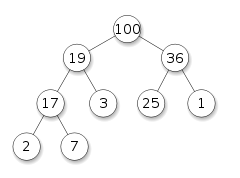
\includegraphics[width=64mm]{heap.png}
\caption{max-heap example borrowed from wikipedia}
\end{figure}

With such heap property, the root node of heap contains the min(max) key value among the whole tree. Operations defined on heap and corresponding time complexity is listed below:

\begin{itemize}
\item insert node with certain key value: $O(\log n)$
\item find node with min(max) key value: $O(1)$
\item update key value of certain node after the node is located: $O(\log n)$
\item remove node with min(max) key value: $O(\log n)$
\end{itemize}

One more thing to mention here is that the complexity of finding node with certain key value should be $O(n)$ in general, since it requires a full scan of the whole data structure. We will play a trick here later.

When implementing heap, we can used an array, named $a$, to represent such tree structure as below:

\begin{figure}[ht]
\centering
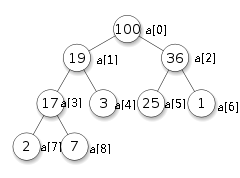
\includegraphics[width=64mm]{heap2.png}
\caption{max-heap example borrowed from wikipedia}
\end{figure}

It's still that example and it can be shown that the two children nodes of node $a[i]$ can be represented as $a[2 \times i + 1]$ and $a[2 \times i + 2]$, if exists.

\subsection{$O(1)$ Find Operation in Heap}

In our specific scenario, the node of heap stands for an alternative with statistic information of its sample values. We used an external array, since the ids of alternatives are natural numbers from $0$ to $k - 1$, to track the internal location, namely the index of the underlay array, of corresponding alternative node inside the heap. It means that we have implemented our own heap which differs from the one in Java standard library to support $O(1)$ complexity query from alternative id to corresponding statistic information.

\subsection{Accelerating Linear Comparison Complexity}

Straightforwardly speaking, when receiving a new sample value of certain alternative in fully sequential R\&S procedure, which cause the update of statistic information of that alternative, we need to carry out a linear complexity comparison, say, comparing this alternatives with every surviving one, to see whether it will eliminate some alternative, or be eliminated by some one else. The linear complexity may be critical when the number of alternatives is extremely large.

After we have customized the heap to support $O(1)$ query in our scenario, we can discuss our $O(\log{n})$ comparison algorithm, digging into the case where we need to select the alternative with minimum mean, since selecting the maximum is quite similar. In this case, alternative i dominates alternative j is equivalent to:

$$ \bar{X}_j(n_j)-\bar{X}_i(n_i) \ge \max\{0,a(\frac{S_i^2}{n_i}+\frac{S_j^2}{n_j}) - b\} $$

From the coding viewpoint, for any updated alternative, which just received an new sample value in fully sequential case, to check whether it dominates other alternatives or be dominated, we need three steps.

Step one is to consider the extreme scenario, although seldom occurs, where $a(\frac{S_i^2}{n_i}+\frac{S_j^2}{n_j}) - b < 0$. To see whether it really happens, just check from the updated alternative and the alternative whose $\frac{S^2}{n}$ is largest among all the alternative except the updated one. If so, one of the two alternatives will be eliminated immediately. For the elimination of the updated alternative, the whole comparing algorithm is done and we can move on directly to next sample value, while for the the elimination of the other one, this step will be repeated. In this way, maintaining a max-heap of alternatives with their $\frac{S^2}{n}$ as sorting key value will save us from looking for the next alternative whose $\frac{S^2}{n}$ is largest among all the survived alternative except the updated one with O(n) time complexity every time repeating this step.

After consideration of extreme scenario, alternative i dominates alternative j only happens when
$$ \bar{X}_j(n_j)-\bar{X}_i(n_i) \ge a(\frac{S_i^2}{n_i}+\frac{S_j^2}{n_j}) - b $$
since for any pair of survived alternatives i and j, $a(\frac{S_i^2}{n_i}+\frac{S_j^2}{n_j}) - b \ge 0$ always holds.

With basic algebra operation, say moving items from one side of equation to the other, the two alternatives can be separated into different sides:

$$ \bar{X}_j(n_j) - a \times \frac{S_j^2}{n_j} \ge \bar{X}_i(n_i) + a \times \frac{S_i^2}{n_i} - b $$

Now is the second step, to see whether the updated alternative dominates any other surviving alternatives, just check from the alternative with largest $\bar{X}(n) - a \times \frac{S^2}{n}$, repeatedly if any elimination happens. This is step two actually and another max-heap of alternatives with $\bar{X}(n) - a \times \frac{S^2}{n}$ as its sorting key value is maintained, for the possibility of repeated elimination.

The third step is even simpler, just checking the survival of the updated alternative against the alternative with smallest $\bar{X}_i(n_i) + a \times \frac{S_i^2}{n_i}$ and no iteration is needed here.

Below is the complete algorithm in fully sequential procedure when processing a new sample value alone:

\begin{algorithm}
 \begin{algorithmic}[1]
 \Require $k, \alpha, \delta, n_0$
 \State $h \gets \text{the Rinott's const with arguments } k, \alpha, n_0$
 \State 
 \While{$r\not=0$}
 \State $a\gets b$
 \State $b\gets r$
 \State $r\gets a\bmod b$
 \EndWhile
 \State \textbf{return} $b$ \Comment{The gcd is b}
 \end{algorithmic}
 \caption{Comparison with One New Sample Value}
 \label{comparsion_one}
\end{algorithm}

During the comparison, time complexity for each possible elimination is $O(\log n)$ , under the condition that locating any certain alternative inside a heap costs less than, at most equal to $O(\log n)$, and this is already satisfied by the customization we have made on standard heap.

\subsection{Numerical Experiment}

In order to focus on the efficiency of comparison part, we used generated sample values loaded from text file. Below is the result, the x-axis stands for the number of processed sample values and the y-axis is the time cost.

\begin{table}[ht]
\begin{center}
\begin{tabular}{|c|c|c|c|c|c|c|}
\hline
Num. of Slaves(n): & 1 & 4 & 8 & 16 & 32 & 48 \\
\hline
Sample Size($\times 10^5$) & 2.426 & 2.434 & 2.442 & 2.442 & 2.433 & 2.436\\
\hline
Elapsed Minutes(t): & 370.5 & 129.4 & 94.4 & 68.3 & 41.7 & 34.2 \\
\hline
\end{tabular} \\
\caption{Performance Data}
\end{center}
\end{table}

The figure shows that our comparing algorithm performs much better than $O(\log n)$ in average. Because if there's no elimination during the comparison, which occurs frequently in experiments, the time complexity will be reduced to $O(1)$, since no adjustment of any data structure is needed. Rigorous algorithm analysis with heap adjustment probability can be regarded as future work.